%%%%%%%%%%%%%%%%%%%%%%%%%%%%%%%%%%%%%%%%%%%%%%%%%%%%%%%%%%
% benchmarks.tex
%%%%%%%%%%%%%%%%%%%%%%%%%%%%%%%%%%%%%%%%%%%%%%%%%%%%%%%%%%

Our system is mainly concerned with optimizing away the overhead that dynamically building and maintaining an X3D scene produces. To show that we have achieved our objective of increasing performance in X3D scenes with only regular nodes and routes (we have not yet profiled external scripts extensively), we have tested the same scene on multiple browsers and profiled the resulting framerates. The browsers we have used are BS Contact and Octaga.

We have tested for scenes with a relatively low number of shapes (300 and 680). We are not really interested in testing the rendering performance, since such a test would mainly compare the efficiency of the underlying rendering APIs and would not be relevant in this context. Both scenes are compared against two other scenes with the same shapes but with 3 \texttt{color interpolators}, 2 \texttt{timers} and 6 \texttt{routes} for each shape. The resulting routing and logic are quite heavy and constitutes a good test the underlying execution model for routes and logical nodes. The tested X3D files are an advanced version of the example seen in Section \ref{sec:case_study}: there is a (rather large) set of shapes, colors and timers and the colors of the shapes are changed according to the timers through heavy use of routes. This benchmark shows how heavy the traditional dynamic model is when handling many routes and large scenes.

Tables 1 through 3 show a comparison in performance for each browser with various hardware configurations; we have compared the performance of our implementation against Octaga and BS Contact, apart from the second testing machine where Octaga had trouble installing and then running at a reasonable speed (to avoid polluting the results we have omitted Octaga from that test):

\begin{table}[htb]\small
\centering
\begin{tabular}{|l|c|c|c|}
\hline
Browser & FPS & FPS (with routes) & Diff \% 	 \\
\hline
\textbf{Test machine 1}  & & & \\
\hline
Ours (300 shapes) & 580 & 510 & -12 \\
Ours (680 shapes) & 265 & 224 & -15 \\
Octaga (300 shapes) &  670 & 340 & -49 \\
Octaga (680 shapes) &  372 & 150 & -60 \\
BS C. (300 shapes) & 370 & 300 & -19 \\
BS C. (680 shapes) & 185 & 145 & -22 \\
\hline
\textbf{Test machine 2}  & & & \\
\hline
Ours (300 shapes) & 670 & 590 & -12 \\
Ours (680 shapes) & 310 & 265 & -15 \\
BS C. (300 shapes) & 530 & 368 & -31 \\
BS C. (680 shapes) & 285 & 146 & -49 \\
\hline
\textbf{Test machine 3}  & & & \\
\hline
Ours (300 shapes) & 640 & 600 & -6 \\
Ours (680 shapes) & 310 & 280 & -10 \\
Octaga (300 shapes) &  720 & 403 & -44 \\
Octaga (680 shapes) &  345 & 181 & -48 \\
BS C. (300 shapes) & 500 & 360 & -28 \\
BS C. (680 shapes) & 215 & 135 & -37 \\
\hline
\end{tabular}
\caption{Test results}
\end{table}

\begin{figure}
\begin{center}
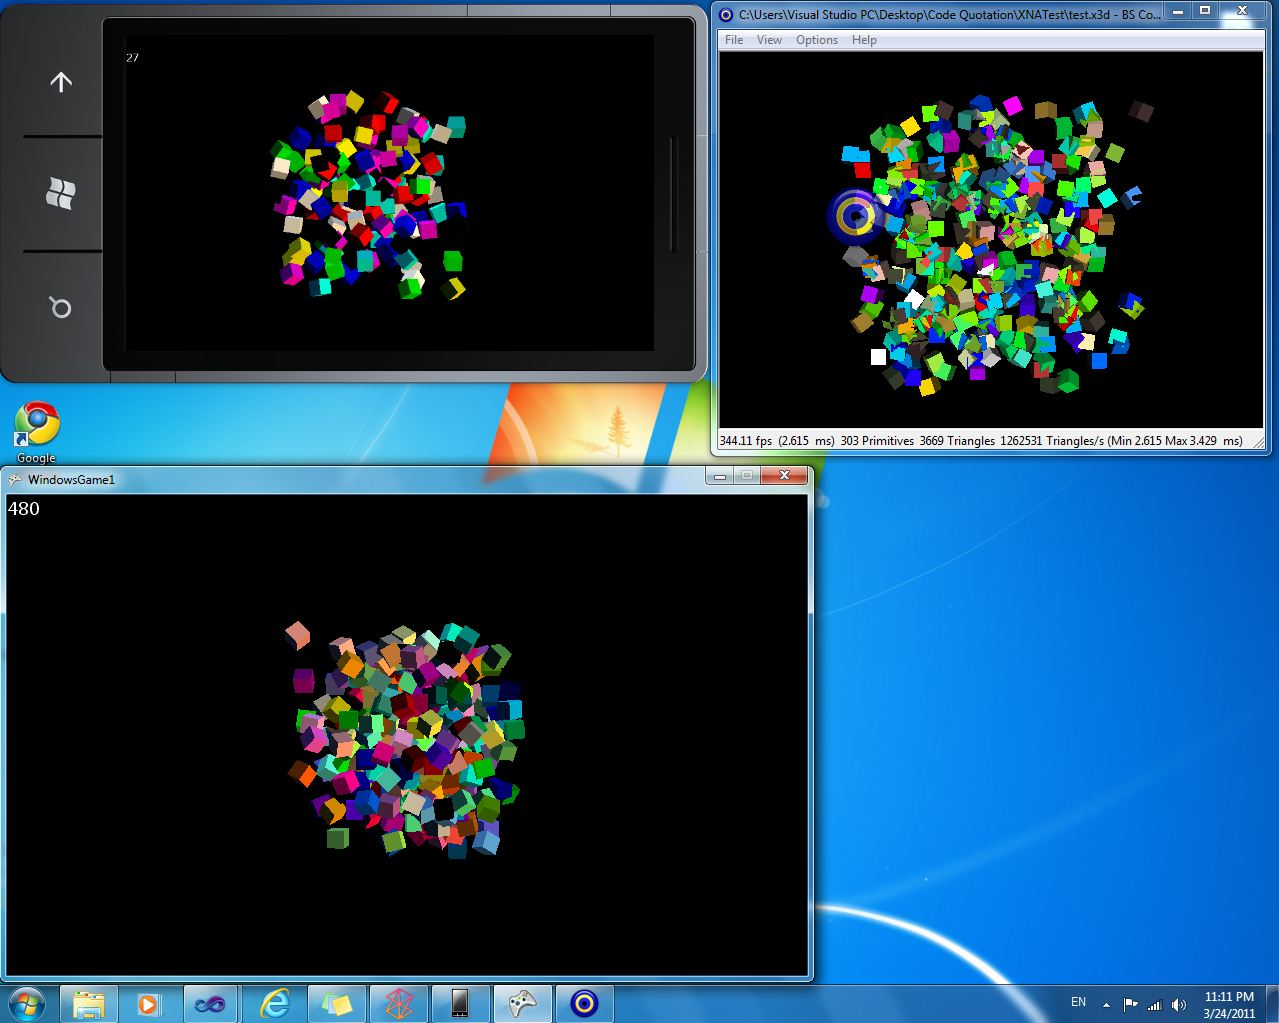
\includegraphics[scale=0.2]{browsers.jpg}
\end{center}
\caption{WP7 Emulator, BS Contact and XNA Windows Application}
\end{figure}

It is clear that thanks to our approach the scene logic weighs far less than it does in the other browsers.

Moreover, as we can see in Figure 3, the code that is generated by our system can be run, \textit{without modification} also in Windows Phone 7 devices; in the figure we can see the same scene run in the Windows Phone 7 emulator (top left), our system (bottom left) and BS Contact (top right). 

Table 4 shows the performance of running, on a Windows Phone 7 device, two compiled scenes with 150 and 300 shapes respectively plus the same routes for each shape used in the tests discussed above. The performance is very good when considered that it is a mobile device; the same technique could be applied to other mobile devices such as iOS or Android, but in our case having used XNA a porting to Windows Phone 7 required literally no effort beyond modifying a compiler switch.

\begin{table}[htb]\small
\centering
\begin{tabular}{|l|c|}
\hline
Scene & FPS 	 \\
\hline
150 shapes with routes & 30 \\
300 shapes with routes & 24 \\
\hline
\end{tabular}
\caption{WP7 (LG Optimus 7)}
\end{table}

At this point we have completed supporting the static aspects of an X3D scene, those that are involved in nodes that are not added or removed dynamically. This approach clearly yields an increase in performance for scenes with a complex logic in terms of timers, routes, interpolators, etc.
